\documentclass[1p]{elsarticle_modified}
%\bibliographystyle{elsarticle-num}

%\usepackage[colorlinks]{hyperref}
%\usepackage{abbrmath_seonhwa} %\Abb, \Ascr, \Acal ,\Abf, \Afrak
\usepackage{amsfonts}
\usepackage{amssymb}
\usepackage{amsmath}
\usepackage{amsthm}
\usepackage{scalefnt}
\usepackage{amsbsy}
\usepackage{kotex}
\usepackage{caption}
\usepackage{subfig}
\usepackage{color}
\usepackage{graphicx}
\usepackage{xcolor} %% white, black, red, green, blue, cyan, magenta, yellow
\usepackage{float}
\usepackage{setspace}
\usepackage{hyperref}

\usepackage{tikz}
\usetikzlibrary{arrows}

\usepackage{multirow}
\usepackage{array} % fixed length table
\usepackage{hhline}

%%%%%%%%%%%%%%%%%%%%%
\makeatletter
\renewcommand*\env@matrix[1][\arraystretch]{%
	\edef\arraystretch{#1}%
	\hskip -\arraycolsep
	\let\@ifnextchar\new@ifnextchar
	\array{*\c@MaxMatrixCols c}}
\makeatother %https://tex.stackexchange.com/questions/14071/how-can-i-increase-the-line-spacing-in-a-matrix
%%%%%%%%%%%%%%%

\usepackage[normalem]{ulem}

\newcommand{\msout}[1]{\ifmmode\text{\sout{\ensuremath{#1}}}\else\sout{#1}\fi}
%SOURCE: \msout is \stkout macro in https://tex.stackexchange.com/questions/20609/strikeout-in-math-mode

\newcommand{\cancel}[1]{
	\ifmmode
	{\color{red}\msout{#1}}
	\else
	{\color{red}\sout{#1}}
	\fi
}

\newcommand{\add}[1]{
	{\color{blue}\uwave{#1}}
}

\newcommand{\replace}[2]{
	\ifmmode
	{\color{red}\msout{#1}}{\color{blue}\uwave{#2}}
	\else
	{\color{red}\sout{#1}}{\color{blue}\uwave{#2}}
	\fi
}

\newcommand{\Sol}{\mathcal{S}} %segment
\newcommand{\D}{D} %diagram
\newcommand{\A}{\mathcal{A}} %arc


%%%%%%%%%%%%%%%%%%%%%%%%%%%%%5 test

\def\sl{\operatorname{\textup{SL}}(2,\Cbb)}
\def\psl{\operatorname{\textup{PSL}}(2,\Cbb)}
\def\quan{\mkern 1mu \triangleright \mkern 1mu}

\theoremstyle{definition}
\newtheorem{thm}{Theorem}[section]
\newtheorem{prop}[thm]{Proposition}
\newtheorem{lem}[thm]{Lemma}
\newtheorem{ques}[thm]{Question}
\newtheorem{cor}[thm]{Corollary}
\newtheorem{defn}[thm]{Definition}
\newtheorem{exam}[thm]{Example}
\newtheorem{rmk}[thm]{Remark}
\newtheorem{alg}[thm]{Algorithm}

\newcommand{\I}{\sqrt{-1}}
\begin{document}

%\begin{frontmatter}
%
%\title{Boundary parabolic representations of knots up to 8 crossings}
%
%%% Group authors per affiliation:
%\author{Yunhi Cho} 
%\address{Department of Mathematics, University of Seoul, Seoul, Korea}
%\ead{yhcho@uos.ac.kr}
%
%
%\author{Seonhwa Kim} %\fnref{s_kim}}
%\address{Center for Geometry and Physics, Institute for Basic Science, Pohang, 37673, Korea}
%\ead{ryeona17@ibs.re.kr}
%
%\author{Hyuk Kim}
%\address{Department of Mathematical Sciences, Seoul National University, Seoul 08826, Korea}
%\ead{hyukkim@snu.ac.kr}
%
%\author{Seokbeom Yoon}
%\address{Department of Mathematical Sciences, Seoul National University, Seoul, 08826,  Korea}
%\ead{sbyoon15@snu.ac.kr}
%
%\begin{abstract}
%We find all boundary parabolic representation of knots up to 8 crossings.
%
%\end{abstract}
%\begin{keyword}
%    \MSC[2010] 57M25 
%\end{keyword}
%
%\end{frontmatter}

%\linenumbers
%\tableofcontents
%
\newcommand\colored[1]{\textcolor{white}{\rule[-0.35ex]{0.8em}{1.4ex}}\kern-0.8em\color{red} #1}%
%\newcommand\colored[1]{\textcolor{white}{ #1}\kern-2.17ex	\textcolor{white}{ #1}\kern-1.81ex	\textcolor{white}{ #1}\kern-2.15ex\color{red}#1	}

{\Large $\underline{11a_{44}~(K11a_{44})}$}

\setlength{\tabcolsep}{10pt}
\renewcommand{\arraystretch}{1.6}
\vspace{1cm}\begin{tabular}{m{100pt}>{\centering\arraybackslash}m{274pt}}
\multirow{5}{120pt}{
	\centering
	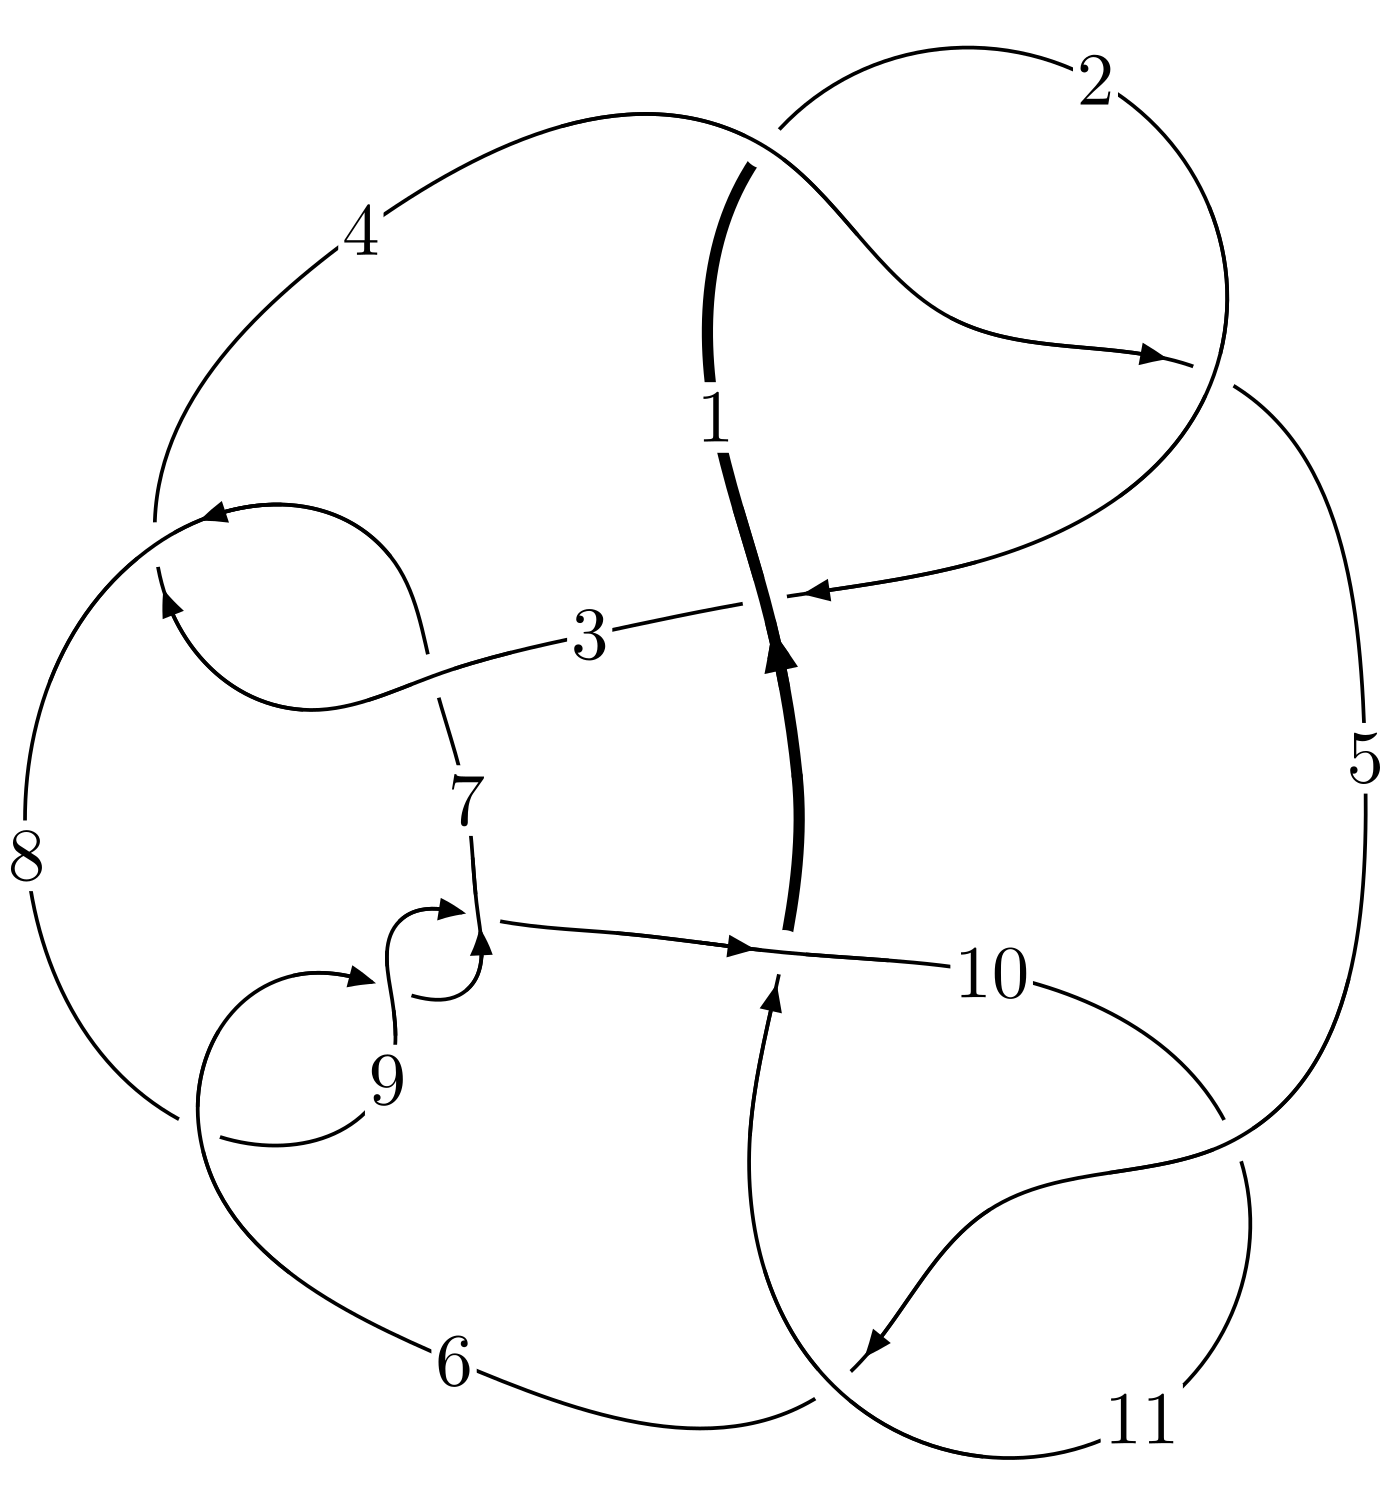
\includegraphics[width=112pt]{../../../GIT/diagram.site/Diagrams/png/293_11a_44.png}\\
\ \ \ A knot diagram\footnotemark}&
\allowdisplaybreaks
\textbf{Linearized knot diagam} \\
\cline{2-2}
 &
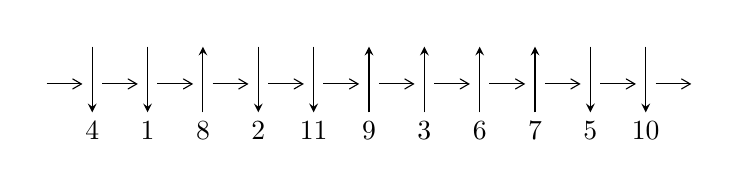
\begin{tikzpicture}[x=20pt, y=17pt]
	% nodes
	\node (C0) at (0, 0) {};
	\node (C1) at (1, 0) {};
	\node (C1U) at (1, +1) {};
	\node (C1D) at (1, -1) {4};

	\node (C2) at (2, 0) {};
	\node (C2U) at (2, +1) {};
	\node (C2D) at (2, -1) {1};

	\node (C3) at (3, 0) {};
	\node (C3U) at (3, +1) {};
	\node (C3D) at (3, -1) {8};

	\node (C4) at (4, 0) {};
	\node (C4U) at (4, +1) {};
	\node (C4D) at (4, -1) {2};

	\node (C5) at (5, 0) {};
	\node (C5U) at (5, +1) {};
	\node (C5D) at (5, -1) {11};

	\node (C6) at (6, 0) {};
	\node (C6U) at (6, +1) {};
	\node (C6D) at (6, -1) {9};

	\node (C7) at (7, 0) {};
	\node (C7U) at (7, +1) {};
	\node (C7D) at (7, -1) {3};

	\node (C8) at (8, 0) {};
	\node (C8U) at (8, +1) {};
	\node (C8D) at (8, -1) {6};

	\node (C9) at (9, 0) {};
	\node (C9U) at (9, +1) {};
	\node (C9D) at (9, -1) {7};

	\node (C10) at (10, 0) {};
	\node (C10U) at (10, +1) {};
	\node (C10D) at (10, -1) {5};

	\node (C11) at (11, 0) {};
	\node (C11U) at (11, +1) {};
	\node (C11D) at (11, -1) {10};
	\node (C12) at (12, 0) {};

	% arrows
	\draw[->,>={angle 60}]
	(C0) edge (C1) (C1) edge (C2) (C2) edge (C3) (C3) edge (C4) (C4) edge (C5) (C5) edge (C6) (C6) edge (C7) (C7) edge (C8) (C8) edge (C9) (C9) edge (C10) (C10) edge (C11) (C11) edge (C12) ;	\draw[->,>=stealth]
	(C1U) edge (C1D) (C2U) edge (C2D) (C3D) edge (C3U) (C4U) edge (C4D) (C5U) edge (C5D) (C6D) edge (C6U) (C7D) edge (C7U) (C8D) edge (C8U) (C9D) edge (C9U) (C10U) edge (C10D) (C11U) edge (C11D) ;
	\end{tikzpicture} \\
\hhline{~~} \\& 
\textbf{Solving Sequence} \\ \cline{2-2} 
 &
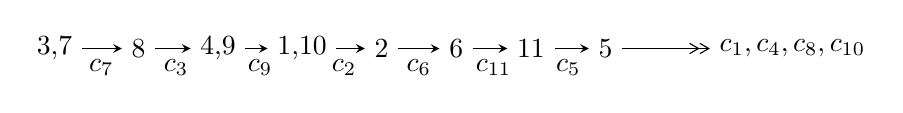
\begin{tikzpicture}[x=27pt, y=7pt]
	% node
	\node (A0) at (-1/8, 0) {3,7};
	\node (A1) at (1, 0) {8};
	\node (A2) at (33/16, 0) {4,9};
	\node (A3) at (51/16, 0) {1,10};
	\node (A4) at (17/4, 0) {2};
	\node (A5) at (21/4, 0) {6};
	\node (A6) at (25/4, 0) {11};
	\node (A7) at (29/4, 0) {5};
	\node (C1) at (1/2, -1) {$c_{7}$};
	\node (C2) at (3/2, -1) {$c_{3}$};
	\node (C3) at (21/8, -1) {$c_{9}$};
	\node (C4) at (15/4, -1) {$c_{2}$};
	\node (C5) at (19/4, -1) {$c_{6}$};
	\node (C6) at (23/4, -1) {$c_{11}$};
	\node (C7) at (27/4, -1) {$c_{5}$};
	\node (A8) at (39/4, 0) {$c_{1},c_{4},c_{8},c_{10}$};

	% edge
	\draw[->,>=stealth]	
	(A0) edge (A1) (A1) edge (A2) (A2) edge (A3) (A3) edge (A4) (A4) edge (A5) (A5) edge (A6) (A6) edge (A7) ;
	\draw[->>,>={angle 60}]	
	(A7) edge (A8);
\end{tikzpicture} \\ 

\end{tabular} \\

\footnotetext{
The image of knot diagram is generated by the software ``\textbf{Draw programme}" developed by Andrew Bartholomew(\url{http://www.layer8.co.uk/maths/draw/index.htm\#Running-draw}), where we modified some parts for our purpose(\url{https://github.com/CATsTAILs/LinksPainter}).
}\phantom \\ \newline 
\centering \textbf{Ideals for irreducible components\footnotemark of $X_{\text{par}}$} 
 
\begin{align*}
I^u_{1}&=\langle 
295797384 u^{18}+418536515 u^{17}+\cdots+3702415268 d-1995040792,\\
\phantom{I^u_{1}}&\phantom{= \langle  }186291706 u^{18}+295294768 u^{17}+\cdots+3702415268 c-4955557140,\\
\phantom{I^u_{1}}&\phantom{= \langle  }-340509075 u^{18}-461083130 u^{17}+\cdots+3702415268 b+2243928812,\\
\phantom{I^u_{1}}&\phantom{= \langle  }-1103288949 u^{18}-1383517078 u^{17}+\cdots+7404830536 a+9000488512,\\
\phantom{I^u_{1}}&\phantom{= \langle  }u^{19}+2 u^{18}+\cdots+4 u^2-8\rangle \\
I^u_{2}&=\langle 
u^7-2 u^6+u^5+3 u^4-5 u^3+3 u^2+d+u-1,\;u^7-3 u^6+u^5+4 u^4-8 u^3+5 u^2+2 c+u-4,\\
\phantom{I^u_{2}}&\phantom{= \langle  }- u^7 a+2 u^6 a+2 u^7-4 u^6-4 u^4 a+2 u^5+5 u^3 a+5 u^4- u^2 a-9 u^3-3 a u+8 u^2+b+2 a- u,\\
\phantom{I^u_{2}}&\phantom{= \langle  }3 u^7 a-4 u^7+\cdots-6 a+8,\;u^8-3 u^7+3 u^6+2 u^5-8 u^4+9 u^3-3 u^2-2 u+2\rangle \\
I^u_{3}&=\langle 
u^5 a+u^4 a- u^5- u^3 a- u^4- u^2 a+u^2+d,\;- u^5 a- u^4 a+u^2 a+u^3+a u+u^2+c-1,\\
\phantom{I^u_{3}}&\phantom{= \langle  }- u^4 a- u^3 a+u^4+2 u^2 a+u^3+a u+b- a- u,\;2 u^5 a+2 u^4 a- u^5-2 u^3 a- u^4-3 u^2 a+a^2+u^2+a,\\
\phantom{I^u_{3}}&\phantom{= \langle  }u^6+u^5- u^4-2 u^3+u+1\rangle \\
I^u_{4}&=\langle 
u^5 c- u^5-2 u^3 c+u^3+2 c u+d- u+1,\;-2 u^4 c- u^3 c+u^4+2 u^2 c+c^2+2 c u- u^2- u,\;- u^2+b,\\
\phantom{I^u_{4}}&\phantom{= \langle  }- u^2+a+1,\;u^6+u^5- u^4-2 u^3+u+1\rangle \\
I^u_{5}&=\langle 
u^5- u^3+d+u,\;2 u^5+2 u^4-3 u^3-4 u^2+c+2 u+2,\;- u^2+b,\;- u^2+a+1,\;u^6+u^5- u^4-2 u^3+u+1\rangle \\
\\
I^v_{1}&=\langle 
a,\;d,\;c-1,\;b-1,\;v+1\rangle \\
I^v_{2}&=\langle 
c,\;d+1,\;b,\;a-1,\;v-1\rangle \\
I^v_{3}&=\langle 
a,\;d+1,\;c- a-1,\;b+1,\;v-1\rangle \\
I^v_{4}&=\langle 
c,\;d+1,\;- a v+c- v-1,\;b v+1\rangle \\
\end{align*}
\raggedright * 8 irreducible components of $\dim_{\mathbb{C}}=0$, with total 68 representations.\\
\raggedright * 1 irreducible components of $\dim_{\mathbb{C}}=1$ \\
\footnotetext{All coefficients of polynomials are rational numbers. But the coefficients are sometimes approximated in decimal forms when there is not enough margin.}
\newpage
\renewcommand{\arraystretch}{1}
\centering \section*{I. $I^u_{1}= \langle 2.96\times10^{8} u^{18}+4.19\times10^{8} u^{17}+\cdots+3.70\times10^{9} d-2.00\times10^{9},\;1.86\times10^{8} u^{18}+2.95\times10^{8} u^{17}+\cdots+3.70\times10^{9} c-4.96\times10^{9},\;-3.41\times10^{8} u^{18}-4.61\times10^{8} u^{17}+\cdots+3.70\times10^{9} b+2.24\times10^{9},\;-1.10\times10^{9} u^{18}-1.38\times10^{9} u^{17}+\cdots+7.40\times10^{9} a+9.00\times10^{9},\;u^{19}+2 u^{18}+\cdots+4 u^2-8 \rangle$}
\flushleft \textbf{(i) Arc colorings}\\
\begin{tabular}{m{7pt} m{180pt} m{7pt} m{180pt} }
\flushright $a_{3}=$&$\begin{pmatrix}0\\u\end{pmatrix}$ \\
\flushright $a_{7}=$&$\begin{pmatrix}1\\0\end{pmatrix}$ \\
\flushright $a_{8}=$&$\begin{pmatrix}1\\- u^2\end{pmatrix}$ \\
\flushright $a_{4}=$&$\begin{pmatrix}u\\- u^3+u\end{pmatrix}$ \\
\flushright $a_{9}=$&$\begin{pmatrix}-0.0503163 u^{18}-0.0797573 u^{17}+\cdots-0.0228247 u+1.33847\\-0.0798931 u^{18}-0.113044 u^{17}+\cdots-0.992877 u+0.538848\end{pmatrix}$ \\
\flushright $a_{1}=$&$\begin{pmatrix}0.148996 u^{18}+0.186840 u^{17}+\cdots+0.656789 u-1.21549\\0.0919694 u^{18}+0.124536 u^{17}+\cdots+1.08046 u-0.606072\end{pmatrix}$ \\
\flushright $a_{10}=$&$\begin{pmatrix}-0.130209 u^{18}-0.192802 u^{17}+\cdots-1.01570 u+1.87731\\-0.0798931 u^{18}-0.113044 u^{17}+\cdots-0.992877 u+0.538848\end{pmatrix}$ \\
\flushright $a_{2}=$&$\begin{pmatrix}0.0237009 u^{18}+0.0450696 u^{17}+\cdots+0.0621551 u-0.293810\\0.0895560 u^{18}+0.0824521 u^{17}+\cdots+1.48819 u-0.554949\end{pmatrix}$ \\
\flushright $a_{6}=$&$\begin{pmatrix}-0.0503163 u^{18}-0.0797573 u^{17}+\cdots-0.0228247 u+1.33847\\0.133048 u^{18}+0.117935 u^{17}+\cdots+1.39541 u-0.705850\end{pmatrix}$ \\
\flushright $a_{11}=$&$\begin{pmatrix}0.106508 u^{18}+0.147732 u^{17}+\cdots+0.953547 u-1.58350\\-0.00966290 u^{18}+0.0305921 u^{17}+\cdots+0.504689 u+0.0161009\end{pmatrix}$ \\
\flushright $a_{5}=$&$\begin{pmatrix}-0.0570264 u^{18}-0.0623040 u^{17}+\cdots+0.423674 u+0.609417\\0.143944 u^{18}+0.132344 u^{17}+\cdots+1.53667 u-1.02006\end{pmatrix}$\\ \flushright $a_{5}=$&$\begin{pmatrix}-0.0570264 u^{18}-0.0623040 u^{17}+\cdots+0.423674 u+0.609417\\0.143944 u^{18}+0.132344 u^{17}+\cdots+1.53667 u-1.02006\end{pmatrix}$\\&\end{tabular}
\flushleft \textbf{(ii) Obstruction class $= -1$}\\~\\
\flushleft \textbf{(iii) Cusp Shapes $= -\frac{1436975081}{1851207634} u^{18}-\frac{348795105}{1851207634} u^{17}+\cdots-\frac{4741127818}{925603817} u+\frac{7721567164}{925603817}$}\\~\\
\newpage\renewcommand{\arraystretch}{1}
\flushleft \textbf{(iv) u-Polynomials at the component}\newline \\
\begin{tabular}{m{50pt}|m{274pt}}
Crossings & \hspace{64pt}u-Polynomials at each crossing \\
\hline $$\begin{aligned}c_{1},c_{4},c_{5}\\c_{10}\end{aligned}$$&$\begin{aligned}
&u^{19}-2 u^{18}+\cdots+3 u-1
\end{aligned}$\\
\hline $$\begin{aligned}c_{2},c_{11}\end{aligned}$$&$\begin{aligned}
&u^{19}+8 u^{18}+\cdots+19 u+1
\end{aligned}$\\
\hline $$\begin{aligned}c_{3},c_{7}\end{aligned}$$&$\begin{aligned}
&u^{19}+2 u^{18}+\cdots+4 u^2-8
\end{aligned}$\\
\hline $$\begin{aligned}c_{6},c_{8},c_{9}\end{aligned}$$&$\begin{aligned}
&u^{19}+2 u^{18}+\cdots-8 u-4
\end{aligned}$\\
\hline
\end{tabular}\\~\\
\newpage\renewcommand{\arraystretch}{1}
\flushleft \textbf{(v) Riley Polynomials at the component}\newline \\
\begin{tabular}{m{50pt}|m{274pt}}
Crossings & \hspace{64pt}Riley Polynomials at each crossing \\
\hline $$\begin{aligned}c_{1},c_{4},c_{5}\\c_{10}\end{aligned}$$&$\begin{aligned}
&y^{19}-8 y^{18}+\cdots+19 y-1
\end{aligned}$\\
\hline $$\begin{aligned}c_{2},c_{11}\end{aligned}$$&$\begin{aligned}
&y^{19}+12 y^{18}+\cdots+195 y-1
\end{aligned}$\\
\hline $$\begin{aligned}c_{3},c_{7}\end{aligned}$$&$\begin{aligned}
&y^{19}-6 y^{18}+\cdots+64 y-64
\end{aligned}$\\
\hline $$\begin{aligned}c_{6},c_{8},c_{9}\end{aligned}$$&$\begin{aligned}
&y^{19}-18 y^{18}+\cdots+88 y-16
\end{aligned}$\\
\hline
\end{tabular}\\~\\
\newpage\flushleft \textbf{(vi) Complex Volumes and Cusp Shapes}
$$\begin{array}{c|c|c}  
\text{Solutions to }I^u_{1}& \I (\text{vol} + \sqrt{-1}CS) & \text{Cusp shape}\\
 \hline 
\begin{aligned}
u &= -1.085440 + 0.040618 I \\
a &= -0.082939 - 0.820035 I \\
b &= -0.548223 - 0.458686 I \\
c &= \phantom{-}0.526397 + 0.204170 I \\
d &= -0.651290 + 0.640476 I\end{aligned}
 & \phantom{-}2.40223 - 3.63220 I & \phantom{-}3.52732 + 6.81616 I \\ \hline\begin{aligned}
u &= -1.085440 - 0.040618 I \\
a &= -0.082939 + 0.820035 I \\
b &= -0.548223 + 0.458686 I \\
c &= \phantom{-}0.526397 - 0.204170 I \\
d &= -0.651290 - 0.640476 I\end{aligned}
 & \phantom{-}2.40223 + 3.63220 I & \phantom{-}3.52732 - 6.81616 I \\ \hline\begin{aligned}
u &= -0.122471 + 1.080680 I \\
a &= \phantom{-}0.718026 + 0.002764 I \\
b &= \phantom{-}1.002700 + 0.800999 I \\
c &= \phantom{-}0.423035 - 0.010382 I \\
d &= -1.362450 - 0.057980 I\end{aligned}
 & \phantom{-}4.14406 - 1.22871 I & \phantom{-}4.10945 + 3.37998 I \\ \hline\begin{aligned}
u &= -0.122471 - 1.080680 I \\
a &= \phantom{-}0.718026 - 0.002764 I \\
b &= \phantom{-}1.002700 - 0.800999 I \\
c &= \phantom{-}0.423035 + 0.010382 I \\
d &= -1.362450 + 0.057980 I\end{aligned}
 & \phantom{-}4.14406 + 1.22871 I & \phantom{-}4.10945 - 3.37998 I \\ \hline\begin{aligned}
u &= \phantom{-}0.583709 + 0.932517 I \\
a &= \phantom{-}1.248640 - 0.243760 I \\
b &= \phantom{-}0.757420 - 1.122890 I \\
c &= \phantom{-}0.663350 - 0.622962 I \\
d &= \phantom{-}0.198964 - 0.752266 I\end{aligned}
 & -4.29720 - 4.85510 I & -5.63265 + 5.33490 I \\ \hline\begin{aligned}
u &= \phantom{-}0.583709 - 0.932517 I \\
a &= \phantom{-}1.248640 + 0.243760 I \\
b &= \phantom{-}0.757420 + 1.122890 I \\
c &= \phantom{-}0.663350 + 0.622962 I \\
d &= \phantom{-}0.198964 + 0.752266 I\end{aligned}
 & -4.29720 + 4.85510 I & -5.63265 - 5.33490 I\\
 \hline 
 \end{array}$$\newpage$$\begin{array}{c|c|c}  
\text{Solutions to }I^u_{1}& \I (\text{vol} + \sqrt{-1}CS) & \text{Cusp shape}\\
 \hline 
\begin{aligned}
u &= -0.628638 + 1.123100 I \\
a &= -1.232770 - 0.120292 I \\
b &= -1.30952 - 1.42851 I \\
c &= \phantom{-}0.413232 - 0.052969 I \\
d &= -1.380830 - 0.305181 I\end{aligned}
 & \phantom{-}0.71510 + 8.68076 I & -0.47305 - 6.48182 I \\ \hline\begin{aligned}
u &= -0.628638 - 1.123100 I \\
a &= -1.232770 + 0.120292 I \\
b &= -1.30952 + 1.42851 I \\
c &= \phantom{-}0.413232 + 0.052969 I \\
d &= -1.380830 + 0.305181 I\end{aligned}
 & \phantom{-}0.71510 - 8.68076 I & -0.47305 + 6.48182 I \\ \hline\begin{aligned}
u &= \phantom{-}1.114960 + 0.705316 I \\
a &= \phantom{-}0.111878 - 1.272940 I \\
b &= -1.46155 - 1.34018 I \\
c &= \phantom{-}0.523314 - 0.396742 I \\
d &= -0.213448 - 0.919956 I\end{aligned}
 & -2.61225 + 10.89710 I & -3.23641 - 8.50579 I \\ \hline\begin{aligned}
u &= \phantom{-}1.114960 - 0.705316 I \\
a &= \phantom{-}0.111878 + 1.272940 I \\
b &= -1.46155 + 1.34018 I \\
c &= \phantom{-}0.523314 + 0.396742 I \\
d &= -0.213448 + 0.919956 I\end{aligned}
 & -2.61225 - 10.89710 I & -3.23641 + 8.50579 I \\ \hline\begin{aligned}
u &= -0.072034 + 0.667244 I \\
a &= -0.502161 - 0.640166 I \\
b &= -0.246691 + 0.049771 I \\
c &= \phantom{-}1.56560 + 0.68284 I \\
d &= \phantom{-}0.463352 + 0.234060 I\end{aligned}
 & -1.32552 + 1.22673 I & -3.58366 - 5.47914 I \\ \hline\begin{aligned}
u &= -0.072034 - 0.667244 I \\
a &= -0.502161 + 0.640166 I \\
b &= -0.246691 - 0.049771 I \\
c &= \phantom{-}1.56560 - 0.68284 I \\
d &= \phantom{-}0.463352 - 0.234060 I\end{aligned}
 & -1.32552 - 1.22673 I & -3.58366 + 5.47914 I\\
 \hline 
 \end{array}$$\newpage$$\begin{array}{c|c|c}  
\text{Solutions to }I^u_{1}& \I (\text{vol} + \sqrt{-1}CS) & \text{Cusp shape}\\
 \hline 
\begin{aligned}
u &= -1.241950 + 0.516338 I \\
a &= \phantom{-}0.276604 + 0.673540 I \\
b &= -1.46152 + 0.68811 I \\
c &= -1.72308 - 0.97561 I \\
d &= \phantom{-}1.43947 - 0.24883 I\end{aligned}
 & \phantom{-}7.80660 - 4.21764 I & \phantom{-}6.24313 + 1.77538 I \\ \hline\begin{aligned}
u &= -1.241950 - 0.516338 I \\
a &= \phantom{-}0.276604 - 0.673540 I \\
b &= -1.46152 - 0.68811 I \\
c &= -1.72308 + 0.97561 I \\
d &= \phantom{-}1.43947 + 0.24883 I\end{aligned}
 & \phantom{-}7.80660 + 4.21764 I & \phantom{-}6.24313 - 1.77538 I \\ \hline\begin{aligned}
u &= \phantom{-}1.391220 + 0.215371 I \\
a &= -0.043768 - 1.017560 I \\
b &= -0.031342 + 0.273386 I \\
c &= -1.88210 + 0.37845 I \\
d &= \phantom{-}1.51067 + 0.10269 I\end{aligned}
 & \phantom{-}9.74824 + 5.99256 I & \phantom{-}5.35093 - 5.49640 I \\ \hline\begin{aligned}
u &= \phantom{-}1.391220 - 0.215371 I \\
a &= -0.043768 + 1.017560 I \\
b &= -0.031342 - 0.273386 I \\
c &= -1.88210 - 0.37845 I \\
d &= \phantom{-}1.51067 - 0.10269 I\end{aligned}
 & \phantom{-}9.74824 - 5.99256 I & \phantom{-}5.35093 + 5.49640 I \\ \hline\begin{aligned}
u &= -1.18800 + 0.79635 I \\
a &= -0.064734 - 1.301180 I \\
b &= \phantom{-}1.97753 - 1.24306 I \\
c &= -1.28148 - 1.20067 I \\
d &= \phantom{-}1.41555 - 0.38935 I\end{aligned}
 & \phantom{-}2.5538 - 15.5977 I & \phantom{-}0.09598 + 9.40344 I \\ \hline\begin{aligned}
u &= -1.18800 - 0.79635 I \\
a &= -0.064734 + 1.301180 I \\
b &= \phantom{-}1.97753 + 1.24306 I \\
c &= -1.28148 + 1.20067 I \\
d &= \phantom{-}1.41555 + 0.38935 I\end{aligned}
 & \phantom{-}2.5538 + 15.5977 I & \phantom{-}0.09598 - 9.40344 I\\
 \hline 
 \end{array}$$\newpage$$\begin{array}{c|c|c}  
\text{Solutions to }I^u_{1}& \I (\text{vol} + \sqrt{-1}CS) & \text{Cusp shape}\\
 \hline 
\begin{aligned}
u &= \phantom{-}0.497291\phantom{ +0.000000I} \\
a &= \phantom{-}0.142445\phantom{ +0.000000I} \\
b &= \phantom{-}0.642422\phantom{ +0.000000I} \\
c &= \phantom{-}0.543479\phantom{ +0.000000I} \\
d &= -0.839998\phantom{ +0.000000I}\end{aligned}
 & \phantom{-}1.20822\phantom{ +0.000000I} & \phantom{-}9.19790\phantom{ +0.000000I}\\
 \hline 
 \end{array}$$\newpage\newpage\renewcommand{\arraystretch}{1}
\centering \section*{II. $I^u_{2}= \langle u^7-2 u^6+\cdots+d-1,\;u^7-3 u^6+\cdots+2 c-4,\;- u^7 a+2 u^7+\cdots+b+2 a,\;3 u^7 a-4 u^7+\cdots-6 a+8,\;u^8-3 u^7+\cdots-2 u+2 \rangle$}
\flushleft \textbf{(i) Arc colorings}\\
\begin{tabular}{m{7pt} m{180pt} m{7pt} m{180pt} }
\flushright $a_{3}=$&$\begin{pmatrix}0\\u\end{pmatrix}$ \\
\flushright $a_{7}=$&$\begin{pmatrix}1\\0\end{pmatrix}$ \\
\flushright $a_{8}=$&$\begin{pmatrix}1\\- u^2\end{pmatrix}$ \\
\flushright $a_{4}=$&$\begin{pmatrix}u\\- u^3+u\end{pmatrix}$ \\
\flushright $a_{9}=$&$\begin{pmatrix}-\frac{1}{2} u^7+\frac{3}{2} u^6+\cdots-\frac{1}{2} u+2\\- u^7+2 u^6- u^5-3 u^4+5 u^3-3 u^2- u+1\end{pmatrix}$ \\
\flushright $a_{1}=$&$\begin{pmatrix}a\\u^7 a-2 u^7+\cdots-2 a+u\end{pmatrix}$ \\
\flushright $a_{10}=$&$\begin{pmatrix}-\frac{3}{2} u^7+\frac{7}{2} u^6+\cdots-\frac{3}{2} u+3\\- u^7+2 u^6- u^5-3 u^4+5 u^3-3 u^2- u+1\end{pmatrix}$ \\
\flushright $a_{2}=$&$\begin{pmatrix}u^6 a+2 u^7+\cdots+3 a-4\\- u^7 a+3 u^6 a+\cdots+2 a-2\end{pmatrix}$ \\
\flushright $a_{6}=$&$\begin{pmatrix}-\frac{1}{2} u^7+\frac{3}{2} u^6+\cdots-\frac{1}{2} u+2\\- u^6+u^5+u^4-3 u^3+2 u^2-1\end{pmatrix}$ \\
\flushright $a_{11}=$&$\begin{pmatrix}- u^7 a+\frac{5}{2} u^7+\cdots+4 a-5\\- u^7+2 u^6+\cdots+2 u-1\end{pmatrix}$ \\
\flushright $a_{5}=$&$\begin{pmatrix}u^7 a-2 u^7+\cdots-3 a+u\\u^7 a- u^6 a+\cdots+u-4\end{pmatrix}$\\ \flushright $a_{5}=$&$\begin{pmatrix}u^7 a-2 u^7+\cdots-3 a+u\\u^7 a- u^6 a+\cdots+u-4\end{pmatrix}$\\&\end{tabular}
\flushleft \textbf{(ii) Obstruction class $= -1$}\\~\\
\flushleft \textbf{(iii) Cusp Shapes $= -2 u^7+4 u^5-6 u^4-4 u^3+6 u^2-8 u-4$}\\~\\
\newpage\renewcommand{\arraystretch}{1}
\flushleft \textbf{(iv) u-Polynomials at the component}\newline \\
\begin{tabular}{m{50pt}|m{274pt}}
Crossings & \hspace{64pt}u-Polynomials at each crossing \\
\hline $$\begin{aligned}c_{1},c_{4},c_{5}\\c_{10}\end{aligned}$$&$\begin{aligned}
&u^{16}- u^{15}+\cdots+4 u-4
\end{aligned}$\\
\hline $$\begin{aligned}c_{2},c_{11}\end{aligned}$$&$\begin{aligned}
&u^{16}+7 u^{15}+\cdots+40 u+16
\end{aligned}$\\
\hline $$\begin{aligned}c_{3},c_{7}\end{aligned}$$&$\begin{aligned}
&(u^8-3 u^7+3 u^6+2 u^5-8 u^4+9 u^3-3 u^2-2 u+2)^2
\end{aligned}$\\
\hline $$\begin{aligned}c_{6},c_{8},c_{9}\end{aligned}$$&$\begin{aligned}
&(u^8+u^7-4 u^6-3 u^5+5 u^4+u^3- u^2+3 u-1)^2
\end{aligned}$\\
\hline
\end{tabular}\\~\\
\newpage\renewcommand{\arraystretch}{1}
\flushleft \textbf{(v) Riley Polynomials at the component}\newline \\
\begin{tabular}{m{50pt}|m{274pt}}
Crossings & \hspace{64pt}Riley Polynomials at each crossing \\
\hline $$\begin{aligned}c_{1},c_{4},c_{5}\\c_{10}\end{aligned}$$&$\begin{aligned}
&y^{16}-7 y^{15}+\cdots-40 y+16
\end{aligned}$\\
\hline $$\begin{aligned}c_{2},c_{11}\end{aligned}$$&$\begin{aligned}
&y^{16}+y^{15}+\cdots-544 y+256
\end{aligned}$\\
\hline $$\begin{aligned}c_{3},c_{7}\end{aligned}$$&$\begin{aligned}
&(y^8-3 y^7+5 y^6-4 y^5+2 y^4-13 y^3+13 y^2-16 y+4)^2
\end{aligned}$\\
\hline $$\begin{aligned}c_{6},c_{8},c_{9}\end{aligned}$$&$\begin{aligned}
&(y^8-9 y^7+32 y^6-53 y^5+31 y^4+15 y^3-15 y^2-7 y+1)^2
\end{aligned}$\\
\hline
\end{tabular}\\~\\
\newpage\flushleft \textbf{(vi) Complex Volumes and Cusp Shapes}
$$\begin{array}{c|c|c}  
\text{Solutions to }I^u_{2}& \I (\text{vol} + \sqrt{-1}CS) & \text{Cusp shape}\\
 \hline 
\begin{aligned}
u &= \phantom{-}0.821613 + 0.567011 I \\
a &= \phantom{-}0.327841 - 1.281680 I \\
b &= -0.32411 - 2.07852 I \\
c &= \phantom{-}0.647330 - 0.378425 I \\
d &= -0.151337 - 0.673064 I\end{aligned}
 & -4.77492 + 2.26376 I & -6.05872 - 4.53378 I \\ \hline\begin{aligned}
u &= \phantom{-}0.821613 + 0.567011 I \\
a &= \phantom{-}1.55977 - 0.26895 I \\
b &= -0.408126 - 1.151440 I \\
c &= \phantom{-}0.647330 - 0.378425 I \\
d &= -0.151337 - 0.673064 I\end{aligned}
 & -4.77492 + 2.26376 I & -6.05872 - 4.53378 I \\ \hline\begin{aligned}
u &= \phantom{-}0.821613 - 0.567011 I \\
a &= \phantom{-}0.327841 + 1.281680 I \\
b &= -0.32411 + 2.07852 I \\
c &= \phantom{-}0.647330 + 0.378425 I \\
d &= -0.151337 + 0.673064 I\end{aligned}
 & -4.77492 - 2.26376 I & -6.05872 + 4.53378 I \\ \hline\begin{aligned}
u &= \phantom{-}0.821613 - 0.567011 I \\
a &= \phantom{-}1.55977 + 0.26895 I \\
b &= -0.408126 + 1.151440 I \\
c &= \phantom{-}0.647330 + 0.378425 I \\
d &= -0.151337 + 0.673064 I\end{aligned}
 & -4.77492 - 2.26376 I & -6.05872 + 4.53378 I \\ \hline\begin{aligned}
u &= \phantom{-}0.432344 + 1.079150 I \\
a &= \phantom{-}1.115680 - 0.168353 I \\
b &= \phantom{-}1.27697 - 0.76242 I \\
c &= \phantom{-}0.420583 + 0.036953 I \\
d &= -1.359440 + 0.207304 I\end{aligned}
 & \phantom{-}2.93531 - 3.55755 I & \phantom{-}2.52739 + 2.62489 I \\ \hline\begin{aligned}
u &= \phantom{-}0.432344 + 1.079150 I \\
a &= -0.603271 + 0.193035 I \\
b &= -0.50994 + 1.48491 I \\
c &= \phantom{-}0.420583 + 0.036953 I \\
d &= -1.359440 + 0.207304 I\end{aligned}
 & \phantom{-}2.93531 - 3.55755 I & \phantom{-}2.52739 + 2.62489 I\\
 \hline 
 \end{array}$$\newpage$$\begin{array}{c|c|c}  
\text{Solutions to }I^u_{2}& \I (\text{vol} + \sqrt{-1}CS) & \text{Cusp shape}\\
 \hline 
\begin{aligned}
u &= \phantom{-}0.432344 - 1.079150 I \\
a &= \phantom{-}1.115680 + 0.168353 I \\
b &= \phantom{-}1.27697 + 0.76242 I \\
c &= \phantom{-}0.420583 - 0.036953 I \\
d &= -1.359440 - 0.207304 I\end{aligned}
 & \phantom{-}2.93531 + 3.55755 I & \phantom{-}2.52739 - 2.62489 I \\ \hline\begin{aligned}
u &= \phantom{-}0.432344 - 1.079150 I \\
a &= -0.603271 - 0.193035 I \\
b &= -0.50994 - 1.48491 I \\
c &= \phantom{-}0.420583 - 0.036953 I \\
d &= -1.359440 - 0.207304 I\end{aligned}
 & \phantom{-}2.93531 + 3.55755 I & \phantom{-}2.52739 - 2.62489 I \\ \hline\begin{aligned}
u &= -1.38845\phantom{ +0.000000I} \\
a &= \phantom{-}0.099908 + 0.914602 I \\
b &= -0.636148 - 0.242515 I \\
c &= -1.96418\phantom{ +0.000000I} \\
d &= \phantom{-}1.50912\phantom{ +0.000000I}\end{aligned}
 & \phantom{-}10.1546\phantom{ +0.000000I} & \phantom{-}6.33750\phantom{ +0.000000I} \\ \hline\begin{aligned}
u &= -1.38845\phantom{ +0.000000I} \\
a &= \phantom{-}0.099908 - 0.914602 I \\
b &= -0.636148 + 0.242515 I \\
c &= -1.96418\phantom{ +0.000000I} \\
d &= \phantom{-}1.50912\phantom{ +0.000000I}\end{aligned}
 & \phantom{-}10.1546\phantom{ +0.000000I} & \phantom{-}6.33750\phantom{ +0.000000I} \\ \hline\begin{aligned}
u &= \phantom{-}1.215250 + 0.684012 I \\
a &= \phantom{-}0.067480 - 1.248660 I \\
b &= -1.57665 - 0.90527 I \\
c &= -1.45820 + 1.13316 I \\
d &= \phantom{-}1.42757 + 0.33227 I\end{aligned}
 & \phantom{-}5.44991 + 9.88301 I & \phantom{-}3.28252 - 6.06963 I \\ \hline\begin{aligned}
u &= \phantom{-}1.215250 + 0.684012 I \\
a &= -0.355893 + 0.630356 I \\
b &= \phantom{-}1.56027 + 1.09581 I \\
c &= -1.45820 + 1.13316 I \\
d &= \phantom{-}1.42757 + 0.33227 I\end{aligned}
 & \phantom{-}5.44991 + 9.88301 I & \phantom{-}3.28252 - 6.06963 I\\
 \hline 
 \end{array}$$\newpage$$\begin{array}{c|c|c}  
\text{Solutions to }I^u_{2}& \I (\text{vol} + \sqrt{-1}CS) & \text{Cusp shape}\\
 \hline 
\begin{aligned}
u &= \phantom{-}1.215250 - 0.684012 I \\
a &= \phantom{-}0.067480 + 1.248660 I \\
b &= -1.57665 + 0.90527 I \\
c &= -1.45820 - 1.13316 I \\
d &= \phantom{-}1.42757 - 0.33227 I\end{aligned}
 & \phantom{-}5.44991 - 9.88301 I & \phantom{-}3.28252 + 6.06963 I \\ \hline\begin{aligned}
u &= \phantom{-}1.215250 - 0.684012 I \\
a &= -0.355893 - 0.630356 I \\
b &= \phantom{-}1.56027 - 1.09581 I \\
c &= -1.45820 - 1.13316 I \\
d &= \phantom{-}1.42757 - 0.33227 I\end{aligned}
 & \phantom{-}5.44991 - 9.88301 I & \phantom{-}3.28252 + 6.06963 I \\ \hline\begin{aligned}
u &= -0.549965\phantom{ +0.000000I} \\
a &= -1.11644\phantom{ +0.000000I} \\
b &= -2.20354\phantom{ +0.000000I} \\
c &= \phantom{-}0.744760\phantom{ +0.000000I} \\
d &= -0.342714\phantom{ +0.000000I}\end{aligned}
 & -2.57083\phantom{ +0.000000I} & \phantom{-}2.16010\phantom{ +0.000000I} \\ \hline\begin{aligned}
u &= -0.549965\phantom{ +0.000000I} \\
a &= -2.30659\phantom{ +0.000000I} \\
b &= \phantom{-}0.439006\phantom{ +0.000000I} \\
c &= \phantom{-}0.744760\phantom{ +0.000000I} \\
d &= -0.342714\phantom{ +0.000000I}\end{aligned}
 & -2.57083\phantom{ +0.000000I} & \phantom{-}2.16010\phantom{ +0.000000I}\\
 \hline 
 \end{array}$$\newpage\newpage\renewcommand{\arraystretch}{1}
\centering \section*{III. $I^u_{3}= \langle u^5 a- u^5+\cdots+u^2+d,\;- u^5 a- u^4 a+\cdots+c-1,\;- u^4 a+u^4+\cdots+b- a,\;2 u^5 a- u^5+\cdots+a^2+a,\;u^6+u^5- u^4-2 u^3+u+1 \rangle$}
\flushleft \textbf{(i) Arc colorings}\\
\begin{tabular}{m{7pt} m{180pt} m{7pt} m{180pt} }
\flushright $a_{3}=$&$\begin{pmatrix}0\\u\end{pmatrix}$ \\
\flushright $a_{7}=$&$\begin{pmatrix}1\\0\end{pmatrix}$ \\
\flushright $a_{8}=$&$\begin{pmatrix}1\\- u^2\end{pmatrix}$ \\
\flushright $a_{4}=$&$\begin{pmatrix}u\\- u^3+u\end{pmatrix}$ \\
\flushright $a_{9}=$&$\begin{pmatrix}u^5 a+u^4 a- u^2 a- u^3- a u- u^2+1\\- u^5 a- u^4 a+u^5+u^3 a+u^4+u^2 a- u^2\end{pmatrix}$ \\
\flushright $a_{1}=$&$\begin{pmatrix}a\\u^4 a+u^3 a- u^4-2 u^2 a- u^3- a u+a+u\end{pmatrix}$ \\
\flushright $a_{10}=$&$\begin{pmatrix}u^5+u^3 a+u^4- u^3- a u-2 u^2+1\\- u^5 a- u^4 a+u^5+u^3 a+u^4+u^2 a- u^2\end{pmatrix}$ \\
\flushright $a_{2}=$&$\begin{pmatrix}- u^3 a+u^4+u^3+a u+2 a- u-1\\u^5 a+u^4 a- u^3 a- u^4-3 u^2 a- u^3+u^2+2 a+u\end{pmatrix}$ \\
\flushright $a_{6}=$&$\begin{pmatrix}u^5 a+u^4 a- u^2 a- u^3- a u- u^2+1\\a u\end{pmatrix}$ \\
\flushright $a_{11}=$&$\begin{pmatrix}u^5 a+u^4 a-2 u^3 a- u^2 a+a u+u^2+2 a-1\\u^5 a+u^4 a- u^3 a- u^4-3 u^2 a- u^3+u^2+2 a+u\end{pmatrix}$ \\
\flushright $a_{5}=$&$\begin{pmatrix}u^4 a+u^3 a- u^4-2 u^2 a- u^3- a u+u\\2 u^4 a-2 u^2 a+2 a-1\end{pmatrix}$\\ \flushright $a_{5}=$&$\begin{pmatrix}u^4 a+u^3 a- u^4-2 u^2 a- u^3- a u+u\\2 u^4 a-2 u^2 a+2 a-1\end{pmatrix}$\\&\end{tabular}
\flushleft \textbf{(ii) Obstruction class $= -1$}\\~\\
\flushleft \textbf{(iii) Cusp Shapes $= -4 u^4+4 u^2+4 u-2$}\\~\\
\newpage\renewcommand{\arraystretch}{1}
\flushleft \textbf{(iv) u-Polynomials at the component}\newline \\
\begin{tabular}{m{50pt}|m{274pt}}
Crossings & \hspace{64pt}u-Polynomials at each crossing \\
\hline $$\begin{aligned}c_{1},c_{4},c_{6}\\c_{8},c_{9}\end{aligned}$$&$\begin{aligned}
&u^{12}+u^{11}-4 u^{10}-2 u^9+7 u^8- u^7-5 u^6+5 u^5- u^4-3 u^3+2 u^2+1
\end{aligned}$\\
\hline $$\begin{aligned}c_{2}\end{aligned}$$&$\begin{aligned}
&u^{12}+9 u^{11}+\cdots-4 u+1
\end{aligned}$\\
\hline $$\begin{aligned}c_{3},c_{7}\end{aligned}$$&$\begin{aligned}
&(u^6+u^5- u^4-2 u^3+u+1)^2
\end{aligned}$\\
\hline $$\begin{aligned}c_{5},c_{10}\end{aligned}$$&$\begin{aligned}
&(u^6- u^5- u^4+2 u^3- u+1)^2
\end{aligned}$\\
\hline $$\begin{aligned}c_{11}\end{aligned}$$&$\begin{aligned}
&(u^6+3 u^5+5 u^4+4 u^3+2 u^2+u+1)^2
\end{aligned}$\\
\hline
\end{tabular}\\~\\
\newpage\renewcommand{\arraystretch}{1}
\flushleft \textbf{(v) Riley Polynomials at the component}\newline \\
\begin{tabular}{m{50pt}|m{274pt}}
Crossings & \hspace{64pt}Riley Polynomials at each crossing \\
\hline $$\begin{aligned}c_{1},c_{4},c_{6}\\c_{8},c_{9}\end{aligned}$$&$\begin{aligned}
&y^{12}-9 y^{11}+\cdots+4 y+1
\end{aligned}$\\
\hline $$\begin{aligned}c_{2}\end{aligned}$$&$\begin{aligned}
&y^{12}-13 y^{11}+\cdots-12 y+1
\end{aligned}$\\
\hline $$\begin{aligned}c_{3},c_{5},c_{7}\\c_{10}\end{aligned}$$&$\begin{aligned}
&(y^6-3 y^5+5 y^4-4 y^3+2 y^2- y+1)^2
\end{aligned}$\\
\hline $$\begin{aligned}c_{11}\end{aligned}$$&$\begin{aligned}
&(y^6+y^5+5 y^4+6 y^2+3 y+1)^2
\end{aligned}$\\
\hline
\end{tabular}\\~\\
\newpage\flushleft \textbf{(vi) Complex Volumes and Cusp Shapes}
$$\begin{array}{c|c|c}  
\text{Solutions to }I^u_{3}& \I (\text{vol} + \sqrt{-1}CS) & \text{Cusp shape}\\
 \hline 
\begin{aligned}
u &= \phantom{-}1.002190 + 0.295542 I \\
a &= \phantom{-}0.228720 - 1.004780 I \\
b &= \phantom{-}0.103539 - 0.942817 I \\
c &= \phantom{-}0.490081 + 0.135670 I \\
d &= -0.895235 + 0.524661 I\end{aligned}
 & \phantom{-}1.89061 + 0.92430 I & \phantom{-}3.71672 - 0.79423 I \\ \hline\begin{aligned}
u &= \phantom{-}1.002190 + 0.295542 I \\
a &= \phantom{-}1.69020 - 0.12901 I \\
b &= -1.18901 - 0.78206 I \\
c &= -2.60446 + 1.12615 I \\
d &= \phantom{-}1.323480 + 0.139870 I\end{aligned}
 & \phantom{-}1.89061 + 0.92430 I & \phantom{-}3.71672 - 0.79423 I \\ \hline\begin{aligned}
u &= \phantom{-}1.002190 - 0.295542 I \\
a &= \phantom{-}0.228720 + 1.004780 I \\
b &= \phantom{-}0.103539 + 0.942817 I \\
c &= \phantom{-}0.490081 - 0.135670 I \\
d &= -0.895235 - 0.524661 I\end{aligned}
 & \phantom{-}1.89061 - 0.92430 I & \phantom{-}3.71672 + 0.79423 I \\ \hline\begin{aligned}
u &= \phantom{-}1.002190 - 0.295542 I \\
a &= \phantom{-}1.69020 + 0.12901 I \\
b &= -1.18901 + 0.78206 I \\
c &= -2.60446 - 1.12615 I \\
d &= \phantom{-}1.323480 - 0.139870 I\end{aligned}
 & \phantom{-}1.89061 - 0.92430 I & \phantom{-}3.71672 + 0.79423 I \\ \hline\begin{aligned}
u &= -0.428243 + 0.664531 I \\
a &= \phantom{-}0.305248 + 0.125739 I \\
b &= -0.101098 + 0.828455 I \\
c &= \phantom{-}0.886780 + 0.510268 I \\
d &= \phantom{-}0.152828 + 0.487477 I\end{aligned}
 & -1.89061 + 0.92430 I & -3.71672 - 0.79423 I \\ \hline\begin{aligned}
u &= -0.428243 + 0.664531 I \\
a &= -0.41743 - 1.68310 I \\
b &= -0.15460 - 3.71488 I \\
c &= \phantom{-}0.460381 - 0.041004 I \\
d &= -1.155020 - 0.191936 I\end{aligned}
 & -1.89061 + 0.92430 I & -3.71672 - 0.79423 I\\
 \hline 
 \end{array}$$\newpage$$\begin{array}{c|c|c}  
\text{Solutions to }I^u_{3}& \I (\text{vol} + \sqrt{-1}CS) & \text{Cusp shape}\\
 \hline 
\begin{aligned}
u &= -0.428243 - 0.664531 I \\
a &= \phantom{-}0.305248 - 0.125739 I \\
b &= -0.101098 - 0.828455 I \\
c &= \phantom{-}0.886780 - 0.510268 I \\
d &= \phantom{-}0.152828 - 0.487477 I\end{aligned}
 & -1.89061 - 0.92430 I & -3.71672 + 0.79423 I \\ \hline\begin{aligned}
u &= -0.428243 - 0.664531 I \\
a &= -0.41743 + 1.68310 I \\
b &= -0.15460 + 3.71488 I \\
c &= \phantom{-}0.460381 + 0.041004 I \\
d &= -1.155020 + 0.191936 I\end{aligned}
 & -1.89061 - 0.92430 I & -3.71672 + 0.79423 I \\ \hline\begin{aligned}
u &= -1.073950 + 0.558752 I \\
a &= \phantom{-}0.266694 + 0.574266 I \\
b &= -1.16959 + 0.91104 I \\
c &= \phantom{-}0.550084 + 0.355577 I \\
d &= -0.282166 + 0.828798 I\end{aligned}
 & \phantom{-0.000000 } -5.69302 I & \phantom{-0.000000 -}0. + 5.51057 I \\ \hline\begin{aligned}
u &= -1.073950 + 0.558752 I \\
a &= -1.57343 - 0.13663 I \\
b &= \phantom{-}1.01075 - 1.59090 I \\
c &= -1.78287 - 1.35197 I \\
d &= \phantom{-}1.356120 - 0.270046 I\end{aligned}
 & \phantom{-0.000000 } -5.69302 I & \phantom{-0.000000 -}0. + 5.51057 I \\ \hline\begin{aligned}
u &= -1.073950 - 0.558752 I \\
a &= \phantom{-}0.266694 - 0.574266 I \\
b &= -1.16959 - 0.91104 I \\
c &= \phantom{-}0.550084 - 0.355577 I \\
d &= -0.282166 - 0.828798 I\end{aligned}
 & \phantom{-0.000000 -}5.69302 I & \phantom{-0.000000 } 0. - 5.51057 I \\ \hline\begin{aligned}
u &= -1.073950 - 0.558752 I \\
a &= -1.57343 + 0.13663 I \\
b &= \phantom{-}1.01075 + 1.59090 I \\
c &= -1.78287 + 1.35197 I \\
d &= \phantom{-}1.356120 + 0.270046 I\end{aligned}
 & \phantom{-0.000000 -}5.69302 I & \phantom{-0.000000 } 0. - 5.51057 I\\
 \hline 
 \end{array}$$\newpage\newpage\renewcommand{\arraystretch}{1}
\centering \section*{IV. $I^u_{4}= \langle u^5 c- u^5+\cdots+d+1,\;-2 u^4 c+u^4+\cdots+c^2- u,\;- u^2+b,\;- u^2+a+1,\;u^6+u^5- u^4-2 u^3+u+1 \rangle$}
\flushleft \textbf{(i) Arc colorings}\\
\begin{tabular}{m{7pt} m{180pt} m{7pt} m{180pt} }
\flushright $a_{3}=$&$\begin{pmatrix}0\\u\end{pmatrix}$ \\
\flushright $a_{7}=$&$\begin{pmatrix}1\\0\end{pmatrix}$ \\
\flushright $a_{8}=$&$\begin{pmatrix}1\\- u^2\end{pmatrix}$ \\
\flushright $a_{4}=$&$\begin{pmatrix}u\\- u^3+u\end{pmatrix}$ \\
\flushright $a_{9}=$&$\begin{pmatrix}c\\- u^5 c+u^5+2 u^3 c- u^3-2 c u+u-1\end{pmatrix}$ \\
\flushright $a_{1}=$&$\begin{pmatrix}u^2-1\\u^2\end{pmatrix}$ \\
\flushright $a_{10}=$&$\begin{pmatrix}- u^5 c+u^5+2 u^3 c- u^3-2 c u+c+u-1\\- u^5 c+u^5+2 u^3 c- u^3-2 c u+u-1\end{pmatrix}$ \\
\flushright $a_{2}=$&$\begin{pmatrix}u^5-2 u^3+u\\u^5- u^3+u\end{pmatrix}$ \\
\flushright $a_{6}=$&$\begin{pmatrix}c\\u^5 c- u^5-2 u^3 c- u^2 c+u^3+2 c u- u+1\end{pmatrix}$ \\
\flushright $a_{11}=$&$\begin{pmatrix}- c\\u^5 c- u^5-2 u^3 c+u^3+2 c u- u+1\end{pmatrix}$ \\
\flushright $a_{5}=$&$\begin{pmatrix}1\\0\end{pmatrix}$\\ \flushright $a_{5}=$&$\begin{pmatrix}1\\0\end{pmatrix}$\\&\end{tabular}
\flushleft \textbf{(ii) Obstruction class $= -1$}\\~\\
\flushleft \textbf{(iii) Cusp Shapes $= -4 u^4+4 u^2+4 u-2$}\\~\\
\newpage\renewcommand{\arraystretch}{1}
\flushleft \textbf{(iv) u-Polynomials at the component}\newline \\
\begin{tabular}{m{50pt}|m{274pt}}
Crossings & \hspace{64pt}u-Polynomials at each crossing \\
\hline $$\begin{aligned}c_{1},c_{4}\end{aligned}$$&$\begin{aligned}
&(u^6- u^5- u^4+2 u^3- u+1)^2
\end{aligned}$\\
\hline $$\begin{aligned}c_{2}\end{aligned}$$&$\begin{aligned}
&(u^6+3 u^5+5 u^4+4 u^3+2 u^2+u+1)^2
\end{aligned}$\\
\hline $$\begin{aligned}c_{3},c_{7}\end{aligned}$$&$\begin{aligned}
&(u^6+u^5- u^4-2 u^3+u+1)^2
\end{aligned}$\\
\hline $$\begin{aligned}c_{5},c_{6},c_{8}\\c_{9},c_{10}\end{aligned}$$&$\begin{aligned}
&u^{12}+u^{11}-4 u^{10}-2 u^9+7 u^8- u^7-5 u^6+5 u^5- u^4-3 u^3+2 u^2+1
\end{aligned}$\\
\hline $$\begin{aligned}c_{11}\end{aligned}$$&$\begin{aligned}
&u^{12}+9 u^{11}+\cdots-4 u+1
\end{aligned}$\\
\hline
\end{tabular}\\~\\
\newpage\renewcommand{\arraystretch}{1}
\flushleft \textbf{(v) Riley Polynomials at the component}\newline \\
\begin{tabular}{m{50pt}|m{274pt}}
Crossings & \hspace{64pt}Riley Polynomials at each crossing \\
\hline $$\begin{aligned}c_{1},c_{3},c_{4}\\c_{7}\end{aligned}$$&$\begin{aligned}
&(y^6-3 y^5+5 y^4-4 y^3+2 y^2- y+1)^2
\end{aligned}$\\
\hline $$\begin{aligned}c_{2}\end{aligned}$$&$\begin{aligned}
&(y^6+y^5+5 y^4+6 y^2+3 y+1)^2
\end{aligned}$\\
\hline $$\begin{aligned}c_{5},c_{6},c_{8}\\c_{9},c_{10}\end{aligned}$$&$\begin{aligned}
&y^{12}-9 y^{11}+\cdots+4 y+1
\end{aligned}$\\
\hline $$\begin{aligned}c_{11}\end{aligned}$$&$\begin{aligned}
&y^{12}-13 y^{11}+\cdots-12 y+1
\end{aligned}$\\
\hline
\end{tabular}\\~\\
\newpage\flushleft \textbf{(vi) Complex Volumes and Cusp Shapes}
$$\begin{array}{c|c|c}  
\text{Solutions to }I^u_{4}& \I (\text{vol} + \sqrt{-1}CS) & \text{Cusp shape}\\
 \hline 
\begin{aligned}
u &= \phantom{-}1.002190 + 0.295542 I \\
a &= -0.082955 + 0.592379 I \\
b &= \phantom{-}0.917045 + 0.592379 I \\
c &= \phantom{-}0.490081 + 0.135670 I \\
d &= -0.895235 + 0.524661 I\end{aligned}
 & \phantom{-}1.89061 + 0.92430 I & \phantom{-}3.71672 - 0.79423 I \\ \hline\begin{aligned}
u &= \phantom{-}1.002190 + 0.295542 I \\
a &= -0.082955 + 0.592379 I \\
b &= \phantom{-}0.917045 + 0.592379 I \\
c &= -2.60446 + 1.12615 I \\
d &= \phantom{-}1.323480 + 0.139870 I\end{aligned}
 & \phantom{-}1.89061 + 0.92430 I & \phantom{-}3.71672 - 0.79423 I \\ \hline\begin{aligned}
u &= \phantom{-}1.002190 - 0.295542 I \\
a &= -0.082955 - 0.592379 I \\
b &= \phantom{-}0.917045 - 0.592379 I \\
c &= \phantom{-}0.490081 - 0.135670 I \\
d &= -0.895235 - 0.524661 I\end{aligned}
 & \phantom{-}1.89061 - 0.92430 I & \phantom{-}3.71672 + 0.79423 I \\ \hline\begin{aligned}
u &= \phantom{-}1.002190 - 0.295542 I \\
a &= -0.082955 - 0.592379 I \\
b &= \phantom{-}0.917045 - 0.592379 I \\
c &= -2.60446 - 1.12615 I \\
d &= \phantom{-}1.323480 - 0.139870 I\end{aligned}
 & \phantom{-}1.89061 - 0.92430 I & \phantom{-}3.71672 + 0.79423 I \\ \hline\begin{aligned}
u &= -0.428243 + 0.664531 I \\
a &= -1.258210 - 0.569162 I \\
b &= -0.258209 - 0.569162 I \\
c &= \phantom{-}0.886780 + 0.510268 I \\
d &= \phantom{-}0.152828 + 0.487477 I\end{aligned}
 & -1.89061 + 0.92430 I & -3.71672 - 0.79423 I \\ \hline\begin{aligned}
u &= -0.428243 + 0.664531 I \\
a &= -1.258210 - 0.569162 I \\
b &= -0.258209 - 0.569162 I \\
c &= \phantom{-}0.460381 - 0.041004 I \\
d &= -1.155020 - 0.191936 I\end{aligned}
 & -1.89061 + 0.92430 I & -3.71672 - 0.79423 I\\
 \hline 
 \end{array}$$\newpage$$\begin{array}{c|c|c}  
\text{Solutions to }I^u_{4}& \I (\text{vol} + \sqrt{-1}CS) & \text{Cusp shape}\\
 \hline 
\begin{aligned}
u &= -0.428243 - 0.664531 I \\
a &= -1.258210 + 0.569162 I \\
b &= -0.258209 + 0.569162 I \\
c &= \phantom{-}0.886780 - 0.510268 I \\
d &= \phantom{-}0.152828 - 0.487477 I\end{aligned}
 & -1.89061 - 0.92430 I & -3.71672 + 0.79423 I \\ \hline\begin{aligned}
u &= -0.428243 - 0.664531 I \\
a &= -1.258210 + 0.569162 I \\
b &= -0.258209 + 0.569162 I \\
c &= \phantom{-}0.460381 + 0.041004 I \\
d &= -1.155020 + 0.191936 I\end{aligned}
 & -1.89061 - 0.92430 I & -3.71672 + 0.79423 I \\ \hline\begin{aligned}
u &= -1.073950 + 0.558752 I \\
a &= -0.158836 - 1.200140 I \\
b &= \phantom{-}0.84116 - 1.20014 I \\
c &= \phantom{-}0.550084 + 0.355577 I \\
d &= -0.282166 + 0.828798 I\end{aligned}
 & \phantom{-0.000000 } -5.69302 I & \phantom{-0.000000 -}0. + 5.51057 I \\ \hline\begin{aligned}
u &= -1.073950 + 0.558752 I \\
a &= -0.158836 - 1.200140 I \\
b &= \phantom{-}0.84116 - 1.20014 I \\
c &= -1.78287 - 1.35197 I \\
d &= \phantom{-}1.356120 - 0.270046 I\end{aligned}
 & \phantom{-0.000000 } -5.69302 I & \phantom{-0.000000 -}0. + 5.51057 I \\ \hline\begin{aligned}
u &= -1.073950 - 0.558752 I \\
a &= -0.158836 + 1.200140 I \\
b &= \phantom{-}0.84116 + 1.20014 I \\
c &= \phantom{-}0.550084 - 0.355577 I \\
d &= -0.282166 - 0.828798 I\end{aligned}
 & \phantom{-0.000000 -}5.69302 I & \phantom{-0.000000 } 0. - 5.51057 I \\ \hline\begin{aligned}
u &= -1.073950 - 0.558752 I \\
a &= -0.158836 + 1.200140 I \\
b &= \phantom{-}0.84116 + 1.20014 I \\
c &= -1.78287 + 1.35197 I \\
d &= \phantom{-}1.356120 + 0.270046 I\end{aligned}
 & \phantom{-0.000000 -}5.69302 I & \phantom{-0.000000 } 0. - 5.51057 I\\
 \hline 
 \end{array}$$\newpage\newpage\renewcommand{\arraystretch}{1}
\centering \section*{V. $I^u_{5}= \langle u^5- u^3+d+u,\;2 u^5+2 u^4+\cdots+c+2,\;- u^2+b,\;- u^2+a+1,\;u^6+u^5- u^4-2 u^3+u+1 \rangle$}
\flushleft \textbf{(i) Arc colorings}\\
\begin{tabular}{m{7pt} m{180pt} m{7pt} m{180pt} }
\flushright $a_{3}=$&$\begin{pmatrix}0\\u\end{pmatrix}$ \\
\flushright $a_{7}=$&$\begin{pmatrix}1\\0\end{pmatrix}$ \\
\flushright $a_{8}=$&$\begin{pmatrix}1\\- u^2\end{pmatrix}$ \\
\flushright $a_{4}=$&$\begin{pmatrix}u\\- u^3+u\end{pmatrix}$ \\
\flushright $a_{9}=$&$\begin{pmatrix}-2 u^5-2 u^4+3 u^3+4 u^2-2 u-2\\- u^5+u^3- u\end{pmatrix}$ \\
\flushright $a_{1}=$&$\begin{pmatrix}u^2-1\\u^2\end{pmatrix}$ \\
\flushright $a_{10}=$&$\begin{pmatrix}-3 u^5-2 u^4+4 u^3+4 u^2-3 u-2\\- u^5+u^3- u\end{pmatrix}$ \\
\flushright $a_{2}=$&$\begin{pmatrix}u^5-2 u^3+u\\u^5- u^3+u\end{pmatrix}$ \\
\flushright $a_{6}=$&$\begin{pmatrix}-2 u^5-2 u^4+3 u^3+4 u^2-2 u-2\\u^3- u\end{pmatrix}$ \\
\flushright $a_{11}=$&$\begin{pmatrix}2 u^5+2 u^4-3 u^3-4 u^2+2 u+2\\u^5- u^3+u\end{pmatrix}$ \\
\flushright $a_{5}=$&$\begin{pmatrix}1\\0\end{pmatrix}$\\ \flushright $a_{5}=$&$\begin{pmatrix}1\\0\end{pmatrix}$\\&\end{tabular}
\flushleft \textbf{(ii) Obstruction class $= -1$}\\~\\
\flushleft \textbf{(iii) Cusp Shapes $= -4 u^4+4 u^2+4 u-2$}\\~\\
\newpage\renewcommand{\arraystretch}{1}
\flushleft \textbf{(iv) u-Polynomials at the component}\newline \\
\begin{tabular}{m{50pt}|m{274pt}}
Crossings & \hspace{64pt}u-Polynomials at each crossing \\
\hline $$\begin{aligned}c_{1},c_{4},c_{5}\\c_{6},c_{8},c_{9}\\c_{10}\end{aligned}$$&$\begin{aligned}
&u^6- u^5- u^4+2 u^3- u+1
\end{aligned}$\\
\hline $$\begin{aligned}c_{2},c_{11}\end{aligned}$$&$\begin{aligned}
&u^6+3 u^5+5 u^4+4 u^3+2 u^2+u+1
\end{aligned}$\\
\hline $$\begin{aligned}c_{3},c_{7}\end{aligned}$$&$\begin{aligned}
&u^6+u^5- u^4-2 u^3+u+1
\end{aligned}$\\
\hline
\end{tabular}\\~\\
\newpage\renewcommand{\arraystretch}{1}
\flushleft \textbf{(v) Riley Polynomials at the component}\newline \\
\begin{tabular}{m{50pt}|m{274pt}}
Crossings & \hspace{64pt}Riley Polynomials at each crossing \\
\hline $$\begin{aligned}c_{1},c_{3},c_{4}\\c_{5},c_{6},c_{7}\\c_{8},c_{9},c_{10}\end{aligned}$$&$\begin{aligned}
&y^6-3 y^5+5 y^4-4 y^3+2 y^2- y+1
\end{aligned}$\\
\hline $$\begin{aligned}c_{2},c_{11}\end{aligned}$$&$\begin{aligned}
&y^6+y^5+5 y^4+6 y^2+3 y+1
\end{aligned}$\\
\hline
\end{tabular}\\~\\
\newpage\flushleft \textbf{(vi) Complex Volumes and Cusp Shapes}
$$\begin{array}{c|c|c}  
\text{Solutions to }I^u_{5}& \I (\text{vol} + \sqrt{-1}CS) & \text{Cusp shape}\\
 \hline 
\begin{aligned}
u &= \phantom{-}1.002190 + 0.295542 I \\
a &= -0.082955 + 0.592379 I \\
b &= \phantom{-}0.917045 + 0.592379 I \\
c &= \phantom{-}0.575561 - 0.267796 I \\
d &= -0.428243 - 0.664531 I\end{aligned}
 & \phantom{-}1.89061 + 0.92430 I & \phantom{-}3.71672 - 0.79423 I \\ \hline\begin{aligned}
u &= \phantom{-}1.002190 - 0.295542 I \\
a &= -0.082955 - 0.592379 I \\
b &= \phantom{-}0.917045 - 0.592379 I \\
c &= \phantom{-}0.575561 + 0.267796 I \\
d &= -0.428243 + 0.664531 I\end{aligned}
 & \phantom{-}1.89061 - 0.92430 I & \phantom{-}3.71672 + 0.79423 I \\ \hline\begin{aligned}
u &= -0.428243 + 0.664531 I \\
a &= -1.258210 - 0.569162 I \\
b &= -0.258209 - 0.569162 I \\
c &= -0.02510 - 3.38343 I \\
d &= \phantom{-}1.002190 - 0.295542 I\end{aligned}
 & -1.89061 + 0.92430 I & -3.71672 - 0.79423 I \\ \hline\begin{aligned}
u &= -0.428243 - 0.664531 I \\
a &= -1.258210 + 0.569162 I \\
b &= -0.258209 + 0.569162 I \\
c &= -0.02510 + 3.38343 I \\
d &= \phantom{-}1.002190 + 0.295542 I\end{aligned}
 & -1.89061 - 0.92430 I & -3.71672 + 0.79423 I \\ \hline\begin{aligned}
u &= -1.073950 + 0.558752 I \\
a &= -0.158836 - 1.200140 I \\
b &= \phantom{-}0.84116 - 1.20014 I \\
c &= \phantom{-}0.449542 - 0.121113 I \\
d &= -1.073950 - 0.558752 I\end{aligned}
 & \phantom{-0.000000 } -5.69302 I & \phantom{-0.000000 -}0. + 5.51057 I \\ \hline\begin{aligned}
u &= -1.073950 - 0.558752 I \\
a &= -0.158836 + 1.200140 I \\
b &= \phantom{-}0.84116 + 1.20014 I \\
c &= \phantom{-}0.449542 + 0.121113 I \\
d &= -1.073950 + 0.558752 I\end{aligned}
 & \phantom{-0.000000 -}5.69302 I & \phantom{-0.000000 } 0. - 5.51057 I\\
 \hline 
 \end{array}$$\newpage\newpage\renewcommand{\arraystretch}{1}
\centering \section*{VI. $I^v_{1}= \langle a,\;d,\;c-1,\;b-1,\;v+1 \rangle$}
\flushleft \textbf{(i) Arc colorings}\\
\begin{tabular}{m{7pt} m{180pt} m{7pt} m{180pt} }
\flushright $a_{3}=$&$\begin{pmatrix}-1\\0\end{pmatrix}$ \\
\flushright $a_{7}=$&$\begin{pmatrix}1\\0\end{pmatrix}$ \\
\flushright $a_{8}=$&$\begin{pmatrix}1\\0\end{pmatrix}$ \\
\flushright $a_{4}=$&$\begin{pmatrix}-1\\0\end{pmatrix}$ \\
\flushright $a_{9}=$&$\begin{pmatrix}1\\0\end{pmatrix}$ \\
\flushright $a_{1}=$&$\begin{pmatrix}0\\1\end{pmatrix}$ \\
\flushright $a_{10}=$&$\begin{pmatrix}1\\0\end{pmatrix}$ \\
\flushright $a_{2}=$&$\begin{pmatrix}-1\\1\end{pmatrix}$ \\
\flushright $a_{6}=$&$\begin{pmatrix}1\\0\end{pmatrix}$ \\
\flushright $a_{11}=$&$\begin{pmatrix}1\\1\end{pmatrix}$ \\
\flushright $a_{5}=$&$\begin{pmatrix}0\\-1\end{pmatrix}$\\ \flushright $a_{5}=$&$\begin{pmatrix}0\\-1\end{pmatrix}$\\&\end{tabular}
\flushleft \textbf{(ii) Obstruction class $= 1$}\\~\\
\flushleft \textbf{(iii) Cusp Shapes $= -12$}\\~\\
\newpage\renewcommand{\arraystretch}{1}
\flushleft \textbf{(iv) u-Polynomials at the component}\newline \\
\begin{tabular}{m{50pt}|m{274pt}}
Crossings & \hspace{64pt}u-Polynomials at each crossing \\
\hline $$\begin{aligned}c_{1},c_{5}\end{aligned}$$&$\begin{aligned}
&u-1
\end{aligned}$\\
\hline $$\begin{aligned}c_{2},c_{4},c_{10}\\c_{11}\end{aligned}$$&$\begin{aligned}
&u+1
\end{aligned}$\\
\hline $$\begin{aligned}c_{3},c_{6},c_{7}\\c_{8},c_{9}\end{aligned}$$&$\begin{aligned}
&u
\end{aligned}$\\
\hline
\end{tabular}\\~\\
\newpage\renewcommand{\arraystretch}{1}
\flushleft \textbf{(v) Riley Polynomials at the component}\newline \\
\begin{tabular}{m{50pt}|m{274pt}}
Crossings & \hspace{64pt}Riley Polynomials at each crossing \\
\hline $$\begin{aligned}c_{1},c_{2},c_{4}\\c_{5},c_{10},c_{11}\end{aligned}$$&$\begin{aligned}
&y-1
\end{aligned}$\\
\hline $$\begin{aligned}c_{3},c_{6},c_{7}\\c_{8},c_{9}\end{aligned}$$&$\begin{aligned}
&y
\end{aligned}$\\
\hline
\end{tabular}\\~\\
\newpage\flushleft \textbf{(vi) Complex Volumes and Cusp Shapes}
$$\begin{array}{c|c|c}  
\text{Solutions to }I^v_{1}& \I (\text{vol} + \sqrt{-1}CS) & \text{Cusp shape}\\
 \hline 
\begin{aligned}
v &= -1.00000\phantom{ +0.000000I} \\
a &= \phantom{-0.000000 } 0 \\
b &= \phantom{-}1.00000\phantom{ +0.000000I} \\
c &= \phantom{-}1.00000\phantom{ +0.000000I} \\
d &= \phantom{-0.000000 } 0\end{aligned}
 & -3.28987\phantom{ +0.000000I} & -12.0000\phantom{ +0.000000I}\\
 \hline 
 \end{array}$$\newpage\newpage\renewcommand{\arraystretch}{1}
\centering \section*{VII. $I^v_{2}= \langle c,\;d+1,\;b,\;a-1,\;v-1 \rangle$}
\flushleft \textbf{(i) Arc colorings}\\
\begin{tabular}{m{7pt} m{180pt} m{7pt} m{180pt} }
\flushright $a_{3}=$&$\begin{pmatrix}1\\0\end{pmatrix}$ \\
\flushright $a_{7}=$&$\begin{pmatrix}1\\0\end{pmatrix}$ \\
\flushright $a_{8}=$&$\begin{pmatrix}1\\0\end{pmatrix}$ \\
\flushright $a_{4}=$&$\begin{pmatrix}1\\0\end{pmatrix}$ \\
\flushright $a_{9}=$&$\begin{pmatrix}0\\-1\end{pmatrix}$ \\
\flushright $a_{1}=$&$\begin{pmatrix}1\\0\end{pmatrix}$ \\
\flushright $a_{10}=$&$\begin{pmatrix}-1\\-1\end{pmatrix}$ \\
\flushright $a_{2}=$&$\begin{pmatrix}1\\0\end{pmatrix}$ \\
\flushright $a_{6}=$&$\begin{pmatrix}1\\1\end{pmatrix}$ \\
\flushright $a_{11}=$&$\begin{pmatrix}0\\-1\end{pmatrix}$ \\
\flushright $a_{5}=$&$\begin{pmatrix}1\\0\end{pmatrix}$\\ \flushright $a_{5}=$&$\begin{pmatrix}1\\0\end{pmatrix}$\\&\end{tabular}
\flushleft \textbf{(ii) Obstruction class $= 1$}\\~\\
\flushleft \textbf{(iii) Cusp Shapes $= 0$}\\~\\
\newpage\renewcommand{\arraystretch}{1}
\flushleft \textbf{(iv) u-Polynomials at the component}\newline \\
\begin{tabular}{m{50pt}|m{274pt}}
Crossings & \hspace{64pt}u-Polynomials at each crossing \\
\hline $$\begin{aligned}c_{1},c_{2},c_{3}\\c_{4},c_{7}\end{aligned}$$&$\begin{aligned}
&u
\end{aligned}$\\
\hline $$\begin{aligned}c_{5},c_{6},c_{11}\end{aligned}$$&$\begin{aligned}
&u+1
\end{aligned}$\\
\hline $$\begin{aligned}c_{8},c_{9},c_{10}\end{aligned}$$&$\begin{aligned}
&u-1
\end{aligned}$\\
\hline
\end{tabular}\\~\\
\newpage\renewcommand{\arraystretch}{1}
\flushleft \textbf{(v) Riley Polynomials at the component}\newline \\
\begin{tabular}{m{50pt}|m{274pt}}
Crossings & \hspace{64pt}Riley Polynomials at each crossing \\
\hline $$\begin{aligned}c_{1},c_{2},c_{3}\\c_{4},c_{7}\end{aligned}$$&$\begin{aligned}
&y
\end{aligned}$\\
\hline $$\begin{aligned}c_{5},c_{6},c_{8}\\c_{9},c_{10},c_{11}\end{aligned}$$&$\begin{aligned}
&y-1
\end{aligned}$\\
\hline
\end{tabular}\\~\\
\newpage\flushleft \textbf{(vi) Complex Volumes and Cusp Shapes}
$$\begin{array}{c|c|c}  
\text{Solutions to }I^v_{2}& \I (\text{vol} + \sqrt{-1}CS) & \text{Cusp shape}\\
 \hline 
\begin{aligned}
v &= \phantom{-}1.00000\phantom{ +0.000000I} \\
a &= \phantom{-}1.00000\phantom{ +0.000000I} \\
b &= \phantom{-0.000000 } 0 \\
c &= \phantom{-0.000000 } 0 \\
d &= -1.00000\phantom{ +0.000000I}\end{aligned}
 & \phantom{-0.000000 } 0 & \phantom{-0.000000 } 0\\
 \hline 
 \end{array}$$\newpage\newpage\renewcommand{\arraystretch}{1}
\centering \section*{VIII. $I^v_{3}= \langle a,\;d+1,\;c- a-1,\;b+1,\;v-1 \rangle$}
\flushleft \textbf{(i) Arc colorings}\\
\begin{tabular}{m{7pt} m{180pt} m{7pt} m{180pt} }
\flushright $a_{3}=$&$\begin{pmatrix}1\\0\end{pmatrix}$ \\
\flushright $a_{7}=$&$\begin{pmatrix}1\\0\end{pmatrix}$ \\
\flushright $a_{8}=$&$\begin{pmatrix}1\\0\end{pmatrix}$ \\
\flushright $a_{4}=$&$\begin{pmatrix}1\\0\end{pmatrix}$ \\
\flushright $a_{9}=$&$\begin{pmatrix}1\\-1\end{pmatrix}$ \\
\flushright $a_{1}=$&$\begin{pmatrix}0\\-1\end{pmatrix}$ \\
\flushright $a_{10}=$&$\begin{pmatrix}0\\-1\end{pmatrix}$ \\
\flushright $a_{2}=$&$\begin{pmatrix}1\\-1\end{pmatrix}$ \\
\flushright $a_{6}=$&$\begin{pmatrix}0\\1\end{pmatrix}$ \\
\flushright $a_{11}=$&$\begin{pmatrix}0\\-1\end{pmatrix}$ \\
\flushright $a_{5}=$&$\begin{pmatrix}0\\1\end{pmatrix}$\\ \flushright $a_{5}=$&$\begin{pmatrix}0\\1\end{pmatrix}$\\&\end{tabular}
\flushleft \textbf{(ii) Obstruction class $= 1$}\\~\\
\flushleft \textbf{(iii) Cusp Shapes $= 0$}\\~\\
\newpage\renewcommand{\arraystretch}{1}
\flushleft \textbf{(iv) u-Polynomials at the component}\newline \\
\begin{tabular}{m{50pt}|m{274pt}}
Crossings & \hspace{64pt}u-Polynomials at each crossing \\
\hline $$\begin{aligned}c_{1},c_{8},c_{9}\end{aligned}$$&$\begin{aligned}
&u-1
\end{aligned}$\\
\hline $$\begin{aligned}c_{2},c_{4},c_{6}\end{aligned}$$&$\begin{aligned}
&u+1
\end{aligned}$\\
\hline $$\begin{aligned}c_{3},c_{5},c_{7}\\c_{10},c_{11}\end{aligned}$$&$\begin{aligned}
&u
\end{aligned}$\\
\hline
\end{tabular}\\~\\
\newpage\renewcommand{\arraystretch}{1}
\flushleft \textbf{(v) Riley Polynomials at the component}\newline \\
\begin{tabular}{m{50pt}|m{274pt}}
Crossings & \hspace{64pt}Riley Polynomials at each crossing \\
\hline $$\begin{aligned}c_{1},c_{2},c_{4}\\c_{6},c_{8},c_{9}\end{aligned}$$&$\begin{aligned}
&y-1
\end{aligned}$\\
\hline $$\begin{aligned}c_{3},c_{5},c_{7}\\c_{10},c_{11}\end{aligned}$$&$\begin{aligned}
&y
\end{aligned}$\\
\hline
\end{tabular}\\~\\
\newpage\flushleft \textbf{(vi) Complex Volumes and Cusp Shapes}
$$\begin{array}{c|c|c}  
\text{Solutions to }I^v_{3}& \I (\text{vol} + \sqrt{-1}CS) & \text{Cusp shape}\\
 \hline 
\begin{aligned}
v &= \phantom{-}1.00000\phantom{ +0.000000I} \\
a &= \phantom{-0.000000 } 0 \\
b &= -1.00000\phantom{ +0.000000I} \\
c &= \phantom{-}1.00000\phantom{ +0.000000I} \\
d &= -1.00000\phantom{ +0.000000I}\end{aligned}
 & \phantom{-0.000000 } 0 & \phantom{-0.000000 } 0\\
 \hline 
 \end{array}$$\newpage\newpage\renewcommand{\arraystretch}{1}
\centering \section*{IX. $I^v_{4}= \langle c,\;d+1,\;- a v+c- v-1,\;b v+1 \rangle$}
\flushleft \textbf{(i) Arc colorings}\\
\begin{tabular}{m{7pt} m{180pt} m{7pt} m{180pt} }
\flushright $a_{3}=$&$\begin{pmatrix}v\\0\end{pmatrix}$ \\
\flushright $a_{7}=$&$\begin{pmatrix}1\\0\end{pmatrix}$ \\
\flushright $a_{8}=$&$\begin{pmatrix}1\\0\end{pmatrix}$ \\
\flushright $a_{4}=$&$\begin{pmatrix}v\\0\end{pmatrix}$ \\
\flushright $a_{9}=$&$\begin{pmatrix}0\\-1\end{pmatrix}$ \\
\flushright $a_{1}=$&$\begin{pmatrix}a\\a+1\end{pmatrix}$ \\
\flushright $a_{10}=$&$\begin{pmatrix}-1\\-1\end{pmatrix}$ \\
\flushright $a_{2}=$&$\begin{pmatrix}a+v\\a+1\end{pmatrix}$ \\
\flushright $a_{6}=$&$\begin{pmatrix}1\\1\end{pmatrix}$ \\
\flushright $a_{11}=$&$\begin{pmatrix}a+1\\a+2\end{pmatrix}$ \\
\flushright $a_{5}=$&$\begin{pmatrix}- a\\- a-1\end{pmatrix}$\\ \flushright $a_{5}=$&$\begin{pmatrix}- a\\- a-1\end{pmatrix}$\\&\end{tabular}
\flushleft \textbf{(ii) Obstruction class $= -1$}\\~\\
\flushleft \textbf{(iii) Cusp Shapes $= - a^2- v^2-2 a-5$}\\~\\
\flushleft \textbf{(iv) u-Polynomials at the component} : It cannot be defined for a positive dimension component.\\~\\
\flushleft \textbf{(v) Riley Polynomials at the component} : It cannot be defined for a positive dimension component.\\~\\
\newpage\flushleft \textbf{(iv) Complex Volumes and Cusp Shapes}
$$\begin{array}{c|c|c} 
\text{Solution to }I^v_{4}& \I (\text{vol} + \sqrt{-1}CS) & \text{Cusp shape}\\
 \hline 
\begin{aligned}
v &= \cdots \\
a &= \cdots \\
b &= \cdots \\
c &= \cdots \\
d &= \cdots\end{aligned}
 & -1.64493\phantom{ +0.000000I} & -3.42386 - 0.27749 I\\
 \hline 
 \end{array}
$$
\newpage\renewcommand{\arraystretch}{1}
\centering \section*{ X. u-Polynomials}
\begin{tabular}{m{50pt}|m{274pt}}
Crossings & \hspace{64pt}u-Polynomials at each crossing \\
\hline $$\begin{aligned}c_{1}\end{aligned}$$&$\begin{aligned}
&u(u-1)^2(u^6- u^5- u^4+2 u^3- u+1)^3\\
&\cdot(u^{12}+u^{11}-4 u^{10}-2 u^9+7 u^8- u^7-5 u^6+5 u^5- u^4-3 u^3+2 u^2+1)\\
&\cdot(u^{16}- u^{15}+\cdots+4 u-4)(u^{19}-2 u^{18}+\cdots+3 u-1)
\end{aligned}$\\
\hline $$\begin{aligned}c_{2},c_{11}\end{aligned}$$&$\begin{aligned}
&u(u+1)^2(u^6+3 u^5+5 u^4+4 u^3+2 u^2+u+1)^3\\
&\cdot(u^{12}+9 u^{11}+\cdots-4 u+1)(u^{16}+7 u^{15}+\cdots+40 u+16)\\
&\cdot(u^{19}+8 u^{18}+\cdots+19 u+1)
\end{aligned}$\\
\hline $$\begin{aligned}c_{3},c_{7}\end{aligned}$$&$\begin{aligned}
&u^3(u^6+u^5- u^4-2 u^3+u+1)^5\\
&\cdot(u^8-3 u^7+3 u^6+2 u^5-8 u^4+9 u^3-3 u^2-2 u+2)^2\\
&\cdot(u^{19}+2 u^{18}+\cdots+4 u^2-8)
\end{aligned}$\\
\hline $$\begin{aligned}c_{4}\end{aligned}$$&$\begin{aligned}
&u(u+1)^2(u^6- u^5- u^4+2 u^3- u+1)^3\\
&\cdot(u^{12}+u^{11}-4 u^{10}-2 u^9+7 u^8- u^7-5 u^6+5 u^5- u^4-3 u^3+2 u^2+1)\\
&\cdot(u^{16}- u^{15}+\cdots+4 u-4)(u^{19}-2 u^{18}+\cdots+3 u-1)
\end{aligned}$\\
\hline $$\begin{aligned}c_{5},c_{10}\end{aligned}$$&$\begin{aligned}
&u(u-1)(u+1)(u^6- u^5- u^4+2 u^3- u+1)^3\\
&\cdot(u^{12}+u^{11}-4 u^{10}-2 u^9+7 u^8- u^7-5 u^6+5 u^5- u^4-3 u^3+2 u^2+1)\\
&\cdot(u^{16}- u^{15}+\cdots+4 u-4)(u^{19}-2 u^{18}+\cdots+3 u-1)
\end{aligned}$\\
\hline $$\begin{aligned}c_{6}\end{aligned}$$&$\begin{aligned}
&u(u+1)^2(u^6- u^5- u^4+2 u^3- u+1)\\
&\cdot(u^8+u^7-4 u^6-3 u^5+5 u^4+u^3- u^2+3 u-1)^2\\
&\cdot(u^{12}+u^{11}-4 u^{10}-2 u^9+7 u^8- u^7-5 u^6+5 u^5- u^4-3 u^3+2 u^2+1)^2\\
&\cdot(u^{19}+2 u^{18}+\cdots-8 u-4)
\end{aligned}$\\
\hline $$\begin{aligned}c_{8},c_{9}\end{aligned}$$&$\begin{aligned}
&u(u-1)^2(u^6- u^5- u^4+2 u^3- u+1)\\
&\cdot(u^8+u^7-4 u^6-3 u^5+5 u^4+u^3- u^2+3 u-1)^2\\
&\cdot(u^{12}+u^{11}-4 u^{10}-2 u^9+7 u^8- u^7-5 u^6+5 u^5- u^4-3 u^3+2 u^2+1)^2\\
&\cdot(u^{19}+2 u^{18}+\cdots-8 u-4)
\end{aligned}$\\
\hline
\end{tabular}\newpage\renewcommand{\arraystretch}{1}
\centering \section*{ XI. Riley Polynomials}
\begin{tabular}{m{50pt}|m{274pt}}
Crossings & \hspace{64pt}Riley Polynomials at each crossing \\
\hline $$\begin{aligned}c_{1},c_{4},c_{5}\\c_{10}\end{aligned}$$&$\begin{aligned}
&y(y-1)^2(y^6-3 y^5+5 y^4-4 y^3+2 y^2- y+1)^3\\
&\cdot(y^{12}-9 y^{11}+\cdots+4 y+1)(y^{16}-7 y^{15}+\cdots-40 y+16)\\
&\cdot(y^{19}-8 y^{18}+\cdots+19 y-1)
\end{aligned}$\\
\hline $$\begin{aligned}c_{2},c_{11}\end{aligned}$$&$\begin{aligned}
&y(y-1)^2(y^6+y^5+5 y^4+6 y^2+3 y+1)^3\\
&\cdot(y^{12}-13 y^{11}+\cdots-12 y+1)(y^{16}+y^{15}+\cdots-544 y+256)\\
&\cdot(y^{19}+12 y^{18}+\cdots+195 y-1)
\end{aligned}$\\
\hline $$\begin{aligned}c_{3},c_{7}\end{aligned}$$&$\begin{aligned}
&y^3(y^6-3 y^5+5 y^4-4 y^3+2 y^2- y+1)^5\\
&\cdot(y^8-3 y^7+5 y^6-4 y^5+2 y^4-13 y^3+13 y^2-16 y+4)^2\\
&\cdot(y^{19}-6 y^{18}+\cdots+64 y-64)
\end{aligned}$\\
\hline $$\begin{aligned}c_{6},c_{8},c_{9}\end{aligned}$$&$\begin{aligned}
&y(y-1)^2(y^6-3 y^5+5 y^4-4 y^3+2 y^2- y+1)\\
&\cdot(y^8-9 y^7+32 y^6-53 y^5+31 y^4+15 y^3-15 y^2-7 y+1)^2\\
&\cdot((y^{12}-9 y^{11}+\cdots+4 y+1)^{2})(y^{19}-18 y^{18}+\cdots+88 y-16)
\end{aligned}$\\
\hline
\end{tabular}
\vskip 2pc
\end{document}